\documentclass[11pt,a4paper]{article}
\usepackage[utf8]{inputenc}
\usepackage[T1]{fontenc}
\usepackage[margin=0.5cm, top=1cm, bottom=1cm]{geometry}
\usepackage[fixed]{fontawesome5} % Option [fixed] pour éviter les conflits
\usepackage{xcolor}
\usepackage{enumitem}
\usepackage{graphicx}

% --- Couleurs (mêmes que ton HTML) ---
\definecolor{sidecolor}{RGB}{52,73,94}    % #34495e
\definecolor{maincolor}{RGB}{44,62,80}    % #2c3e50
\definecolor{accentcolor}{RGB}{52,152,219} % #3498db
\definecolor{lightgray}{RGB}{245,245,245} % #f5f5f5

% --- Styles ---
\pagestyle{empty}
\setlength{\parindent}{0pt}
\setlength{\parskip}{6pt}

% --- Barres de compétences (sans tikz) ---
\newcommand{\skillbar}[1]{%
  \colorbox{lightgray}{\rule{10em}{0.2em}}%
  \colorbox{accentcolor}{\rule{#1em}{0.2em}}%
}

\begin{document}

% --- En-tête ---
\begin{center}
  \colorbox{maincolor}{%
    \parbox{\dimexpr\textwidth-2\fboxsep\relax}{%
      \color{white}\centering
      {\Huge\bfseries PRÉNOM NOM\par}
      \vspace{4pt}
      {\Large Poste actuel | Spécialisation\par}
    }%
  }%
\end{center}

% --- Contenu principal (2 colonnes) ---
\vspace{10pt}
\begin{minipage}[t]{0.3\textwidth}
  % --- Photo ---
  \begin{center}
    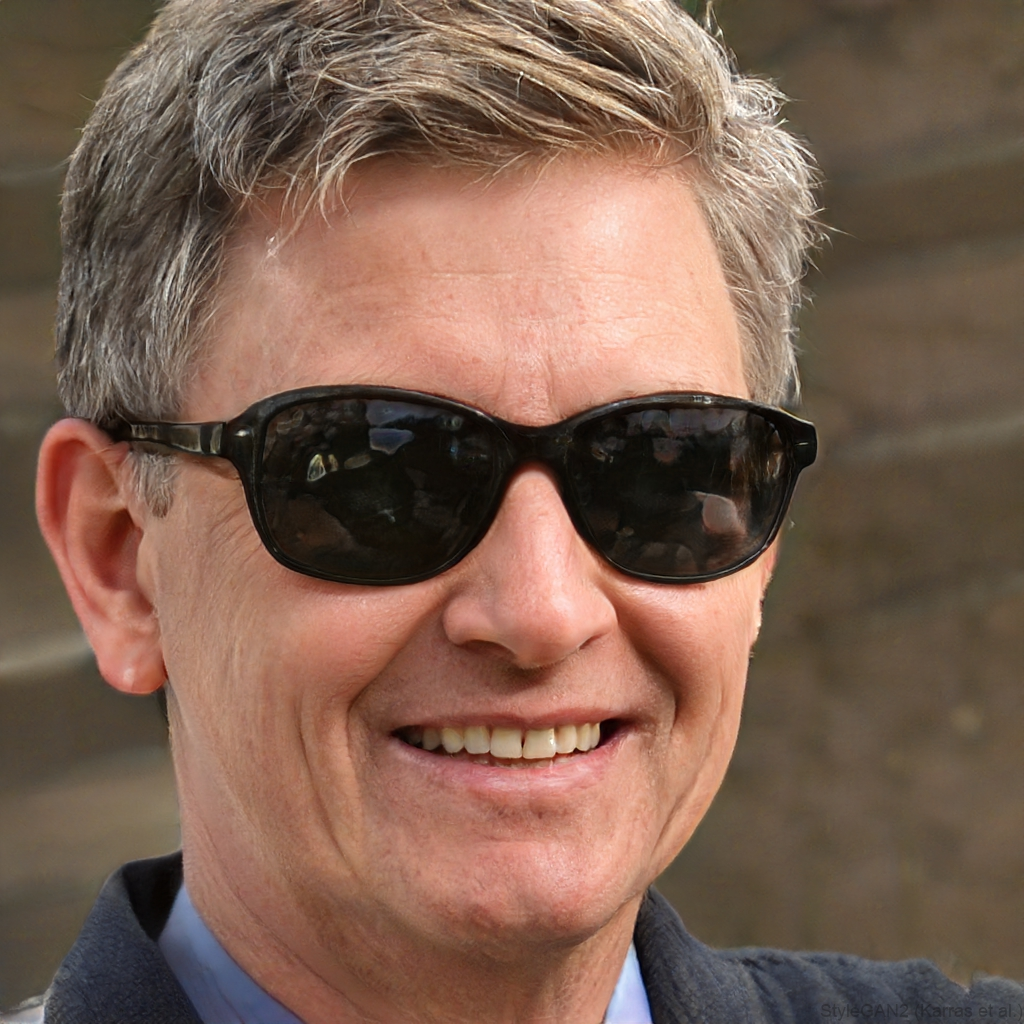
\includegraphics[width=3cm]{thispersondoesnotexist.jpg} % Remplace par ta photo
  \end{center}

  % --- Informations ---
  \vspace{10pt}
  \colorbox{sidecolor}{%
    \parbox{\dimexpr\linewidth-2\fboxsep\relax}{%
      \color{white}
      \vspace{10pt}
      \textbf{\large INFORMATIONS}\par
      \hrulefill\par
      \vspace{5pt}
      \faMapMarkerAlt~ Adresse, Ville, Pays\par
      \faPhone~ +XX XXX XXX XXX\par
      \faEnvelope~ email@domaine.com\par
      \faGlobe~ www.monsite.com\par
      \faLinkedin~ linkedin.com/in/profil\par

      \vspace{10pt}
      \textbf{\large COMPÉTENCES}\par
      \hrulefill\par
      \vspace{5pt}
      Compétence 1\par\skillbar{9}\par
      Compétence 2\par\skillbar{8}\par
      Compétence 3\par\skillbar{7}\par

      \vspace{10pt}
      \textbf{\large LANGUES}\par
      \hrulefill\par
      \vspace{5pt}
      Français : Courant\par
      Anglais : Intermédiaire\par

      \vspace{10pt}
      \textbf{\large ATOUTS}\par
      \hrulefill\par
      \vspace{5pt}
      \begin{itemize}[nosep,leftmargin=*]
        \item Orienté résultats
        \item Esprit d'équipe
        \item Autonome et rigoureux
      \end{itemize}
      \vspace{10pt}
    }%
  }%
\end{minipage}%
\hfill
\begin{minipage}[t]{0.68\textwidth}
  % --- Profil ---
  \textbf{\large PROFIL}\par
  \colorbox{accentcolor}{\rule{\linewidth}{1pt}}\par
  \vspace{5pt}
  Professionnel motivé avec X années d'expérience dans [domaine]. Spécialisé dans [compétences clés]. Passionné par [centres d'intérêt professionnels].\par

  \vspace{10pt}
  % --- Expérience ---
  \textbf{\large EXPÉRIENCE PROFESSIONNELLE}\par
  \colorbox{accentcolor}{\rule{\linewidth}{1pt}}\par
  \vspace{5pt}

  \textbf{Poste occupé} \hfill MM/AAAA – Présent\par
  \textit{Entreprise, Ville}\par
  \begin{itemize}[nosep,leftmargin=*]
    \item Réalisation de [tâche principale 1] avec [résultat quantifiable].
    \item Gestion de [tâche principale 2] pour [bénéfice].
    \item Collaboration avec [équipes/partenaires] sur [projet].
  \end{itemize}

  \vspace{10pt}
  \textbf{Poste précédent} \hfill MM/AAAA – MM/AAAA\par
  \textit{Entreprise précédente, Ville}\par
  \begin{itemize}[nosep,leftmargin=*]
    \item Responsable de [tâche principale 1].
    \item Développement de [compétence/projet].
  \end{itemize}

  \vspace{10pt}
  % --- Formation ---
  \textbf{\large FORMATION}\par
  \colorbox{accentcolor}{\rule{\linewidth}{1pt}}\par
  \vspace{5pt}

  \textbf{Diplôme obtenu} \hfill AAAA – AAAA\par
  \textit{École/Université, Ville}\par
  Spécialisation en [domaine]. Mémoire sur [sujet].\par

  \vspace{10pt}
  % --- Certifications ---
  \textbf{\large CERTIFICATIONS}\par
  \colorbox{accentcolor}{\rule{\linewidth}{1pt}}\par
  \vspace{5pt}

  \textbf{Certification obtenue} \hfill 2026\par
  \textit{Organisme}\par
  Cyber X\par

  \vspace{10pt}
  % --- Domaines d'expertise ---
  \textbf{\large DOMAINES D'EXPERTISE}\par
  \colorbox{accentcolor}{\rule{\linewidth}{1pt}}\par
  \vspace{5pt}

  \textbf{Standards \& Réglementations}\par
  RGPD, ISO 27001, 27002, 27005, EBIOS RM, NIS2, DORA, CRA\par
\end{minipage}

% --- Pied de page ---
\vfill
\begin{center}
  \footnotesize\textcolor{gray}{CV généré avec LaTeX | Optimisé pour ATS}
\end{center}

% --- Version ATS (texte brut) ---
\clearpage
\section*{Version optimisée pour les ATS}
\textbf{Prénom NOM} \\
Poste actuel | Spécialisation en cybersécurité, conformité RGPD, ISO 27001, NIS2, DORA \\
\\
\textbf{Expérience Professionnelle} \\
\textbf{Poste occupé} chez Entreprise (MM/AAAA – Présent) : Gestion des risques, audit, conformité, RGPD, ISO 27001. \\
\textbf{Poste précédent} chez Entreprise précédente (MM/AAAA – MM/AAAA) : Mise en place de politiques de sécurité. \\
\\
\textbf{Formation} \\
\textbf{Diplôme obtenu} à École (AAAA – AAAA) en [domaine]. \\
\\
\textbf{Compétences} \\
RGPD, ISO 27001, ISO 27002, ISO 27005, EBIOS RM, NIS2, DORA, CRA, Cybersécurité, Audit, Gestion des risques, SIEM, Firewalls \\
\\
\textbf{Langues} \\
Français (courant), Anglais (intermédiaire) \\
\\
\textbf{Certifications} \\
Cyber X (2026)

\end{document}